%%% Local Variables:
%%% mode: latex
%%% TeX-master: "wafomanual"
%%% End:
%\svnInfo $Id: standardizedSpectra.tex 667 2011-03-11 11:12:46Z georg $
%
\chapter{Standardized wave spectra}
\label{cha:waveSpectra}
Knowledge of which kind of spectral density is suitable to describe
sea state data are well established from experimental studies.
Qualitative considerations of wave measurements indicate that the
spectra may be divided into 3 parts, (see Fig.~\ref{fig:qspecvar20}):
\begin{enumerate}\setlength\itemsep{0mm}
\item Sea states dominated by wind sea but significantly influenced
by swell components.
\item More or less pure wind seas or, possibly, swell component
  located well inside the wind frequency band.
\item Sea states more or less dominated by swell but significantly
influenced by wind sea.
\end{enumerate}
\begin{figure}[ht!]
 \begin{minipage}[b]{\linewidth}%
  \begin{center}
    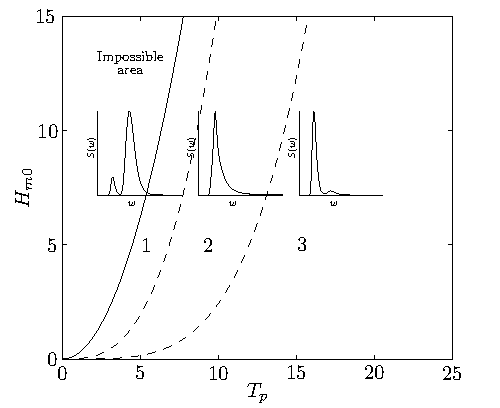
\includegraphics[width=4in]{qspecvar1}
   % \input{qspecvar.tex}
\vspace{-3mm}
\caption[Qualitative indication of spectral variability]
{Qualitative indication of spectral variability.} %
    \label{fig:qspecvar20} %
    % \caption{A LaPrint figure}
    % \label{fig:fig1}
  \end{center}
 \end{minipage}
\end{figure}

One often uses some parametric form of the spectral density. The three
most important parametric spectral densities implemented in
\progname{} will be
described in the following sections.

\section{{\sc Jonswap} spectrum}
\label{sec:jonswap}
The {\sc Jonswap} (JOint North Sea WAve Project) spectrum of
\cite{HasselmannEtal1973Measurements}  is a result of a
multinational project to characterize standardized wave spectra for
the Southeast part of the North Sea. The spectrum is valid for not
fully developed sea states. However, it is also used to represent
fully developed sea states. It is particularly well suited to
characterize wind sea when $3.6 \sqrt{H_{m0}} < T_{p} < 5 \sqrt{H_{m0}}$.
The {\sc Jonswap} spectrum is given in the form:
 \begin{align}
   S^{+}(\w) &= \frac{\alpha \, g^{2}}{\w^{M}}
   \exp \Big( -\frac{M}{N} \, \big(   \frac{\w_{p}}{\w} \big)^{N} \Big) \,
   \gamma^{\exp \Big( \frac{-(\w / \w_{p}-1)^{2}}{2 \, \sigma^{2}} \Big)},  \label{eq:jonswap} \\
\intertext{where}
\sigma &=  \begin{cases}
     0.07 & \text{if} \; \w < \w_{p}, \\
     0.09 & \text{if} \; \w \ge \w_{p},
    \end{cases} \nonumber \\
  M &= 5, \quad  N = 4, \nonumber \\
  \alpha &\approx 5.061 \frac{H_{m0}^{2}}{T_{p}^{4}} \,\Big\{ 1-0.287\, \ln(\gamma)  \Big\}. \nonumber
 \end{align}

A standard value for the peakedness parameter, $\gamma$, is
$3.3$. However, a more correct approach is
to relate $\gamma$ to $H_{m0}$ and $T_{p}$, and use
\begin{gather}
  \gamma = \exp \Big\{3.484 \,\big(1-0.1975\,(0.036-0.0056\,T_{p}/\sqrt{H_{m0}})
\,T_{p}^{4}/H_{m0}^2\big) \Big\} .
%\intertext{where}
% D = 0.036-0.0056\,T_{p}/\sqrt{H_{m0}}
\end{gather}
Here $\gamma$ is limited by $1 \le \gamma \le 7$.
This parameterization is based on qualitative considerations of deep water
wave data from the North Sea; see
\cite{TorsethaugenEtal1984Characteristica} and \cite{HaverAndNyhus1986Wave}.

The relation between the peak period and mean zero-upcrossing period
may be approximated by
\begin{equation}
   T_{m02} \approx T_{p}/\left(1.30301-0.01698\,\gamma+0.12102/\gamma \right)
\end{equation}
The {\sc Jonswap} spectrum is identical with the two-parameter
Pierson-Moskowitz, Bretschneider,
ITTC (International Towing Tank Conference) or ISSC (International Ship and
Offshore Structures Congress) wave spectrum, given $H_{m0}$ and
$T_{p}$, when $\gamma=1$. (For more properties of this spectrum, see the \progname{} function
\verb+jonswap.m+.
\index[xcmds]{{\tt jonswap}}\index[xentr]{ISSC}\index[xcmds]{{\tt bretschneider}}
\index[xentr]{Pierson-Moskowitz}\index[xcmds]{{\tt pmspec}}

\section{Torsethaugen spectrum}
\label{sec:torsethaugen}
Torsethaugen,
\cite{Torsethaugen1993Two,Torsethaugen1994Model,Torsethaugen1996Model},
proposed to
describe bimodal spectra by
%a superposition of two modified {\sc Jonswap} spectra for
%the swell and the wind peak, respectively:
\begin{gather}
 S^{+}(\w) = \sum_{i=1}^{2} S_{J}^{+}(\w;H_{m0,i},\w_{p,i},\gamma_{i},N_{i},M_{i},\alpha_{i})
\end{gather}
where $S_{J}^{+}$ is the {\sc Jonswap} spectrum defined by
Eq.~(\ref{eq:jonswap}). The parameters
$H_{m0,\,i}$, $\w_{p,\,i}$, $N_{i}$, $M_{i}$,
and $\alpha_{i}$ for $i=1,2$, are the
significant wave height, angular peak frequency,
spectral shape and normalization
parameters for the primary and secondary peak, respectively.
\index[xcmds]{{\tt torsethaugen}}\index[xcmds]{{\tt jonswap}}

 These parameters are fitted to
%classes of $H_{m0}$ and $T_{p}$,originating from a dataset consisting
%of
20 000 spectra divided into 146 different classes of $H_{m0}$ and
$T_{p}$ obtained
%The Datasets were measured
at the  Statfjord field in the North Sea in the period from 1980 to 1989.
 The  measured  $H_{m0}$ and $T_{p}$ values for the data
 range from $0.5$ to $11$ meters and from $3.5$ to $19$ seconds, respectively.

Given $H_{m0}$ and $T_{p}$ these parameters are found by the following steps.
The borderline between wind dominated and swell dominated sea states
is defined by the fully developed sea, for which
\begin{equation}
T_{p} = T_{f} = 6.6 \, H_{m0}^{1/3},
\end{equation}
while for $T_{p} < T_{f}$, the local wind sea dominates the spectral peak,
and if $T_{p} > T_{f}$, the swell peak is dominating.

For each of the three types a non-dimensional period scale is introduced by
\begin{align*}
\epsilon_{l\,u} &= \frac{T_{f}-T_{p}}{T_{f}-T_{lu}},
\intertext{where}
T_{lu} &=
\begin{cases}
     2 \, \sqrt{H_{m0}} & \text{if} \; T_{p} \le T_{f} \quad
     \text{(Lower limit)},\\
     25 & \text{if} \; T_{p} > T_{f} \quad
     \text{(Upper limit)},
    \end{cases}
\intertext{defines the lower or upper value for $T_{p}$.
The significant wave height for each peak is given as}
H_{m0,1} &= R_{pp} \, H_{m0} \quad  H_{m0,2} = \sqrt{1-R_{pp}^{2}} \, H_{m0},
\intertext{where}
R_{pp} &= \big(1-A_{10}\big) \,\exp\Big(-\big(\frac{\epsilon_{l\,u}}{A_{1}}
\big)^{2} \Big) +A_{10}, \\
%\label{eq:A-values}
A_{1} &= \begin{cases}
   0.5 & \text{if} \; T_{p} \le T_{f}, \\
   0.3 & \text{if} \; T_{p} > T_{f},
    \end{cases} \quad
A_{10} = \begin{cases}
   0.7 & \text{if} \; T_{p} \le T_{f}, \\
   0.6 & \text{if} \; T_{p} > T_{f}.
    \end{cases}
\end{align*}

The primary and secondary peak periods are defined as
\begin{align*}
T_{p,\,1} &= T_{p}, \\
T_{p,\,2} &=
\begin{cases}
    T_{f} + 2  & \text{if} \; T_{p} \le T_{f}, \\[0.3em]
    \left( \frac{M_{2}\,(N_{2}/M_{2})^{(N_{2}-1)/M_{2}}/\Gamma((N_{2}-1)/M_{2} )}
    {1.28\,(0.4)^{N_{2}} \{1-\exp (-H_{m0,\,2}/3)
      \} } \right)^{1/(N_{2}-1)} & \text{if} \; T_{p} > T_{f},
\end{cases}
\intertext{where the spectral shape parameters are given as}
N_{1} &= N_{2} = 0.5\, \sqrt{H_{m0}}+3.2, \\
M_{i} &=  \begin{cases}
4\, \Big( 1-0.7\exp
\big(\frac{-H_{m0}}{3}\big)\Big) & \text{if} \; T_{p} > T_{f} \;
\text{and} \; i=2, \\
4 & \text{otherwise}.
  \end{cases}
\end{align*}

The peakedness parameters are defined as
\begin{align*}
\gamma_{1} &= 35 \,\Big(1+3.5\, \exp \big( -H_{m0} \big)\Big) \gamma_{T}, \qquad \gamma_{2} = 1,
\intertext{where}
\gamma_{T} &= \begin{cases}
\Big( \frac{2 \, \pi \, H_{m0,\,1}}{g \, T_{p}^{2}}\Big)^{0.857} & \text{if} \; T_{p} \le T_{f}, \\
\big(1+6\,\epsilon_{lu}\big) \Big( \frac{2 \,  \pi \, H_{m0}}{g \, T_{f}^{2}}\Big)^{0.857} & \text{if} \; T_{p} > T_{f}.
    \end{cases}
\end{align*}

Finally the normalization parameters $\alpha_{i}$ ($i=1,2$) are found by numerical
integration so that
\begin{align*}
\int_{0}^{\infty}
S_{J}^{+}(\w;H_{m0,i},\w_{p,i},\gamma_{i},N_{i},M_{i},\alpha_{i})\,d\w
= H_{m0,\,i}^{2}/16.
\end{align*}
 Preliminary comparisons with spectra from other areas indicate that
 the empirical parameters in the Torsethaugen spectrum can be
 dependent on geographical location.
 This spectrum is implemented as a matlab function
 \verb+torsethaugen.m+ in the \progname{} toolbox.

\section{Ochi-Hubble spectrum}
\label{sec:ochi-hubble}
Ochi and Hubble \cite{OchiAndHubble1976Six}, suggested to describe bimodal spectra by a
superposition of two modified Bretschneider (Pierson-Moskovitz)
spectra:
\index[xcmds]{{\tt ochi-hubble}}\index[xcmds]{{\tt bretschneider}}
 \begin{align*}   \label{eq:ohspec1} %
   S^{+}(\w) &=\frac{1}{4} \sum_{i=1}^{2}
   \frac{\big( \big( \lambda_{i}+1/4 \big) \, \w_{p,\,i}^{4}
\big)^{\lambda_{i}}}{\Gamma(\lambda_{i})}
   \frac{H_{m0,\,i}^{2}}{\w^{4 \, \lambda_{i}}+1}
   \exp \Big( \frac{-\big( \lambda_{i}+1/4 \big) \, \w_{p,\,i}^{4}}{\w^{4}}\Big),
 \end{align*}
where $H_{m0,\,i}$, $\w_{p,\,i}$, and $\lambda_{i}$ for $i=1,2$, are
significant wave height, angular peak frequency, and spectral shape
parameter for the low and high frequency components, respectively.

 The values of these parameters are determined from an analysis of data
 obtained in the North Atlantic. The source of the data is the same as
 that for the development of the Pierson-Moskowitz spectrum, but
 analysis is carried out on over $800$ spectra including those in
 partially developed seas and those having a bimodal shape.
In contrast to the {\sc Jonswap}  and Torsethaugen spectra, which are
parameterized as function of $H_{m0}$ and $T_{p}$, Ochi and Hubble,
\cite{OchiAndHubble1976Six} gave, from a
 statistical analysis of the data, a family of wave spectra consisting
 of 11 members generated for a desired sea severity ($H_{m0}$) with the
 coefficient of $0.95$.

The values of the six parameters as functions of $H_{m0}$ are given as:
\begin{align*}
 H_{m0,1} &= R_{p,1} \, H_{m0}, \\
 H_{m0,2} &= \sqrt{1-R_{p,1}^{2}} \, H_{m0}, \\
 \w_{p,i} &= a_{i}\,\exp \big( -b_{i}\, H_{m0} \big), \\
 \lambda_{i} &= c_{i}\,\exp \big( -d_{i}\, H_{m0} \big),
\end{align*}
where $d_{1}=0$ and the remaining empirical constants $a_{i}$, $b_{i}$
($i=1,2$), and $d_{2}$, are given in Table~\ref{tab:oh-parameters}.
(See also the function \verb+ochihubble.m+ in the \progname{} toolbox.)

\begin{table}[htbp]
  \begin{center}
    \begin{tabular}{| c | c c c c c c c c |} \hline \hline
Member no. & $R_{p,1}$ & $a_{1}$ & $a_{2}$ & $b_{1}$ & $b_{2}$ & $c_{1}$ & $c_{2}$ & $d_{2}$ \\ \hline
1  & 0.84 & 0.70 & 1.15 & 0.046 & 0.039 & 3.00 & 1.54 & 0.062 \\
2  & 0.84 & 0.93 & 1.50 & 0.056 & 0.046 & 3.00 & 2.77 & 0.112 \\
3  & 0.84 & 0.41 & 0.88 & 0.016 & 0.026 & 2.55 & 1.82 & 0.089 \\
4  & 0.84 & 0.74 & 1.30 & 0.052 & 0.039 & 2.65 & 3.90 & 0.085 \\
5  & 0.84 & 0.62 & 1.03 & 0.039 & 0.030 & 2.60 & 0.53 & 0.069 \\
6  & 0.95 & 0.70 & 1.50 & 0.046 & 0.046 & 1.35 & 2.48 & 0.102 \\
7  & 0.65 & 0.61 & 0.94 & 0.039 & 0.036 & 4.95 & 2.48 & 0.102 \\
8  & 0.90 & 0.81 & 1.60 & 0.052 & 0.033 & 1.80 & 2.95 & 0.105 \\
9  & 0.77 & 0.54 & 0.61 & 0.039 & 0.000 & 4.50 & 1.95 & 0.082 \\
10 & 0.73 & 0.70 & 0.99 & 0.046 & 0.039 & 6.40 & 1.78 & 0.069 \\
11 & 0.92 & 0.70 & 1.37 & 0.046 & 0.039 & 0.70 & 1.78 & 0.069 \\ \hline \hline
    \end{tabular}
    \caption[Empirical parameter values for the Ochi-Hubble spectral model]
{Empirical parameter values for the Ochi-Hubble spectral model.}
    \label{tab:oh-parameters}
  \end{center}
\end{table}
Member no.~1 given in Table~\ref{tab:oh-parameters} defines the most
  probable spectrum, while member no.~2 to 11 define the $0.95$ percent
  confidence spectra.

  A significant advantage of using a family of spectra for design  of
 marine systems is that one of the family members yields the largest
 response such as motions or wave induced forces for a specified sea
 severity, while anothers yield the smallest response with confidence
 coefficient of $0.95$.

Rodrigues and Soares
\cite{RodriguezAndSoares2000Wave}, used the Ochi-Hubble spectrum with
9 different parameterizations representing
 3 types of sea state categories: swell
dominated (a), wind sea dominated (b) and mixed wind sea and swell
system with comparable energy (c).
Each category is represented by 3 different inter-modal distances between
the swell and the wind sea spectral components.
These three subgroups are denoted by I, II and III, respectively.
The exact values for the six parameters  are given in
Table~\ref{tab:soares-param}. (See the function
\verb+ohspec3.m+ in the \progname{} toolbox.)

  \begin{table}[htbp]
    \begin{center}
      \begin{tabular}{|c | c  |c c c c c c|} \hline \hline
% \multicolumn{2}{|c|}{} &  \multicolumn{6}{|c|}{Target spectra parameters} \\ \hline
 \shortstack{Sea state\\ type} & \shortstack{Sea state \\group} &
 $H_{m0,\,1}$ & $H_{m0,\,2}$ & $\w_{p,\,1}$ &    $\w_{p,\,2}$  &
 $\lambda_{1}$ &   $\lambda_{2}$ \\  \hline
  &   I & 5.5  &   3.5  &   0.440  &   0.691  &   3.0  &  6.5 \\
a &  II & 6.5  &   2.0  &   0.440  &   0.942  &   3.5  &  4.0 \\
  & III & 5.5  &   3.5  &   0.283  &   0.974  &   3.0  &  6.0 \\ \hline
  &   I & 2.0  &   6.5  &   0.440  &   0.691  &   3.0  &  6.5 \\
b &  II & 2.0  &   6.5  &   0.440  &   0.942  &   4.0  &  3.5 \\
  & III & 2.0  &   6.5  &   0.283  &   0.974  &   2.0  &  7.0 \\ \hline
  &   I & 4.1  &   5.0  &   0.440  &   0.691  &   2.1  &  2.5 \\
c &  II & 4.1  &   5.0  &   0.440  &   0.942  &   2.1  &  2.5 \\
  & III & 4.1  &   5.0  &   0.283  &   0.974  &   2.1  &  2.5 \\  \hline \hline
      \end{tabular}
      \caption[Target spectra parameters for mixed sea states ~~]
{Target spectra parameters for mixed sea states.}
      \label{tab:soares-param}
    \end{center}
  \end{table}


%\bibliography{refer}
%\bibliographystyle{apalike20}
%\addcontentsline{toc}{section}{References}
%\bibliographystyle{chicago2}

%%% Local Variables:
%%% mode: latex
%%% TeX-master: "wafomanual"
%%% End:
